% ============================================================
%  Partie 2 — Intégration des Covariables Environnementales
% ============================================================

\chapter{Partie 2 — Intégration de covariables environnementales}
\label{chap:partie2}

\section{Introduction}

L'objectif de cette seconde phase est de pallier les limites de la discrimination
purement spectrale en intégrant des données exogènes. La Partie~1 a établi un
pipeline de classification basé exclusivement sur les séries temporelles Sentinel-2.
La Partie~2 enrichit ce cadre en adjoignant trois groupes de covariables
environnementales~: climatiques (ERA5), pédologiques (OpenLandMap) et
topographiques (ETOPO1/ALOS). L'objectif est double~: (i) mesurer l'apport de
chaque groupe de covariables via une ablation study systématique, et (ii) valider
la généralisation du modèle sur les deux régions géographiques étudiées en Partie~1.

% ============================================================
\section{Présentation et justification des covariables}

Sept covariables environnementales ont été retenues, structurées en trois catégories.

\begin{table}[H]
\centering
\small
\begin{tabular}{|l|l|l|l|}
\hline
\textbf{Catégorie} & \textbf{Covariable} & \textbf{Source} & \textbf{Unité / Format} \\ \hline
\multirow{3}{*}{\textbf{Pédologie (Sol)}}
  & pH (\texttt{ph\_b0})               & OpenLandMap & pH réel ($\div$10) \\ \cline{2-4}
  & Carbone Organique (\texttt{oc\_b0}) & OpenLandMap & g/kg ($\div$5)     \\ \cline{2-4}
  & Texture (\texttt{texture\_b0})      & OpenLandMap & Classe USDA (1--12) \\ \hline
\multirow{2}{*}{\textbf{Topographie}}
  & Élévation (\texttt{elevation})      & ETOPO1 (NOAA) & Mètres \\ \cline{2-4}
  & Modelé (\texttt{landforms})         & ALOS (CSP/ERGo) & Catégoriel entier \\ \hline
\multirow{3}{*}{\textbf{Climat}}
  & Température moyenne (\texttt{T\_c}) & ERA5 Daily & °C \\ \cline{2-4}
  & Précipitations (\texttt{P\_mm})     & ERA5 Daily & mm \\ \cline{2-4}
  & Humidité Relative (\texttt{RH})     & ERA5 Daily & \% \\ \hline
\end{tabular}
\caption{Récapitulatif des covariables environnementales intégrées au modèle.}
\label{tab:covariables}
\end{table}

\subsection{Justification scientifique}

\textbf{1. Propriétés du sol (\texttt{soil})~:} Le pH, le carbone organique et la
texture sont retenus pour leur rôle déterminant dans l'aptitude des terres agricoles.
La cartographie du carbone organique constitue un indicateur clé de la santé des
sols~\cite{ou2024}. Ces variables imposent des contraintes biophysiques directes~:
le riz tolère des sols argileux acides là où le soja nécessite des sols neutres~\cite{tufail2025}.

\textbf{2. Variables climatiques (\texttt{clim})~:} La température, les précipitations
et l'humidité relative pilotent la phénologie des cultures. Ces facteurs dictent les
cycles de croissance et influencent directement la réponse spectrale captée par
Sentinel-2~\cite{wang2024}. L'humidité, étroitement liée aux précipitations, est
par ailleurs un facteur critique pour la modélisation par réseaux de neurones~\cite{jiao2025}.

\textbf{3. Topographie (\texttt{topo})~:} L'élévation et les modelés du terrain
permettent de distinguer les contextes de drainage et les microclimats locaux
(zones de bas-fonds \textit{vs} plateaux), essentiels pour la précision des cartes
de cultures à grande échelle~\cite{adrah2025}.

% ============================================================
\section{Exploration des données}

\subsection{Distribution des covariables statiques par région}

\begin{figure}[H]
    \centering
    \begin{subfigure}[b]{0.48\textwidth}
        \centering
        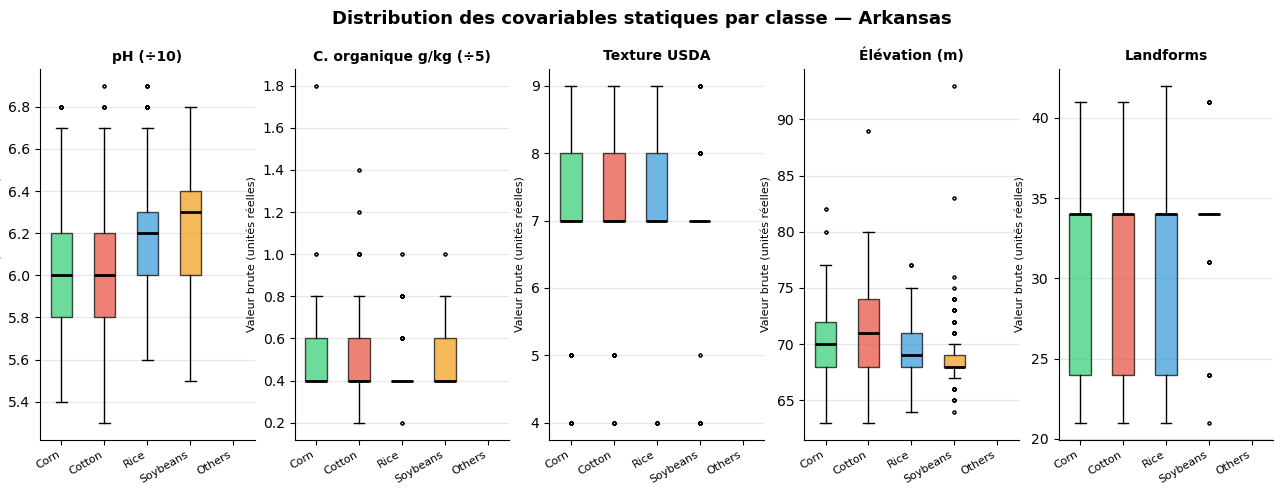
\includegraphics[width=\textwidth]{figures/distribution_covariable_arkansas.png}
        \caption{Arkansas}
        \label{fig:cov_arkansas}
    \end{subfigure}
    \hfill
    \begin{subfigure}[b]{0.48\textwidth}
        \centering
        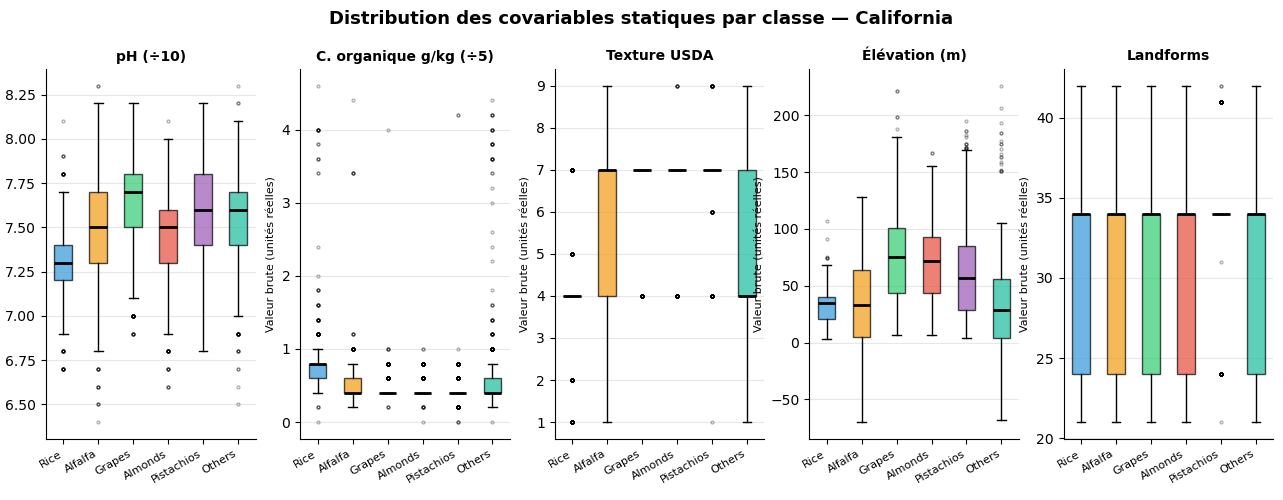
\includegraphics[width=\textwidth]{figures/distribution_covariable_california.png}
        \caption{California}
        \label{fig:cov_california}
    \end{subfigure}
    \caption{Distribution des covariables statiques (pH, carbone organique, texture USDA,
    élévation et landforms) par classe de culture pour les deux régions.}
    \label{fig:covariables}
\end{figure}

\subsubsection*{Arkansas (Figure~\ref{fig:cov_arkansas})}

Les cinq cultures analysées en Arkansas (maïs, coton, riz, soja, autres) présentent des
profils pédologiques relativement homogènes. Le pH varie entre 5{,}5 et 6{,}5 pour la
majorité des classes, traduisant des sols légèrement acides typiques des plaines alluviales.
Le carbone organique est faible pour toutes les cultures (médiane $\approx 0{,}4$--$0{,}6$~g/kg),
avec peu de dispersion. La texture USDA est dominée par des valeurs autour de 7--8,
correspondant à des limons argileux. L'élévation est globalement basse et homogène (65--95~m),
reflétant la topographie plane du delta du Mississippi. Les \textit{landforms} montrent
peu de variabilité inter-classes (25--35), confirmant un terrain peu accidenté.

\subsubsection*{Californie (Figure~\ref{fig:cov_california})}

La Californie présente une plus grande hétérogénéité entre classes. Le pH est plus élevé
(7{,}0--8{,}0), reflétant des sols plus alcalins caractéristiques des vallées irriguées.
Le carbone organique reste faible mais avec davantage de valeurs aberrantes, notamment pour
la luzerne (\textit{Alfalfa}) et la catégorie \textit{Others}. La texture USDA est très
variable selon les cultures. L'élévation est nettement plus dispersée (de $-50$ à $+200$~m),
traduisant la diversité topographique de l'État entre plaines côtières et vallées intérieures.

\medskip
\noindent\textbf{Synthèse.} Ces distributions suggèrent que les covariables statiques ont
un pouvoir discriminant limité en Arkansas en raison de l'homogénéité des conditions
pédoclimatiques, alors qu'en Californie, l'élévation et la texture constituent des
variables potentiellement plus informatives.

% ============================================================
\section{Prétraitement des covariables}

\subsection{Extraction et conversions d'unités}

Les colonnes climatiques sont détectées dynamiquement par préfixe~:
\texttt{T\_c\_*} (température), \texttt{P\_mm\_*} (précipitations), \texttt{RH\_*}
(humidité relative), produisant $36 \times 3 = 108$ dimensions pour les variables
climatiques. Les colonnes statiques \texttt{ph\_b0}, \texttt{oc\_b0},
\texttt{texture\_b0}, \texttt{elevation} et \texttt{landforms} sont extraites par nom.

Deux conversions d'unités physiques fixes sont appliquées avant toute normalisation~:

\begin{itemize}
    \item \textbf{pH du sol} (\texttt{ph\_b0})~: valeurs brutes encodées en pH~$\times 10$.
    Division par 10 pour ramener à l'unité réelle~: $\texttt{ph\_b0} \leftarrow \texttt{ph\_b0} / 10$
    \item \textbf{Carbone organique} (\texttt{oc\_b0})~: valeurs brutes en dg/kg.
    Division par 5 pour convertir en g/kg~: $\texttt{oc\_b0} \leftarrow \texttt{oc\_b0} / 5$
\end{itemize}

Le vecteur de covariables complet résulte de la concaténation des trois groupes~:
\[
    \mathbf{c} = \left[\,\mathbf{c}_{\text{clim}} \;\|\; \mathbf{s}_{\text{sol}}
    \;\|\; \mathbf{s}_{\text{topo}}\,\right] \in \mathbb{R}^{113}
    \quad (108 + 3 + 2)
\]

Sept configurations sont évaluées dans l'ablation study~: \texttt{soil} ($K=3$),
\texttt{clim} ($K=108$), \texttt{topo} ($K=2$), \texttt{clim\_soil} ($K=111$),
\texttt{clim\_topo} ($K=110$), \texttt{soil\_topo} ($K=5$) et \texttt{all} ($K=113$).

\subsection{Stratégie de split et normalisation}
\label{sec:split_norm}

Le pipeline suit strictement l'ordre suivant pour éviter toute fuite de données~:

\begin{enumerate}
    \item \textbf{Split sur données brutes.} Pour chaque classe,
    $\min(300, |\mathcal{C}|)$ individus sont sélectionnés aléatoirement (graine fixée
    à 42), puis répartis en train~(80\,\%) et val~(20\,\%). Les individus restants
    constituent le jeu de test.
    \item \textbf{Fit du \texttt{StandardScaler} sur le train uniquement.}
    \[
        \hat{c}_k = \frac{c_k - \mu_k^{\text{train}}}{\sigma_k^{\text{train}}}
    \]
    \item \textbf{Transform appliqué sur val et test} avec le même scaler, sans re-fit.
    \item \textbf{Sauvegarde du scaler} en \texttt{.pkl} pour inférence future.
\end{enumerate}

\subsection{Fichiers de sortie}

\begin{table}[H]
\centering
\begin{tabular}{lll}
\hline
\textbf{Fichier} & \textbf{Forme} & \textbf{Description} \\
\hline
\texttt{*\_input1.npy}             & $(N, 10, 36)$ & Bandes S2 normalisées ($\div 10\,000$) \\
\texttt{*\_input2.npy}             & $(N, 36)$     & Masque données manquantes $\{0,1\}$ \\
\texttt{*\_covars\_all.npy}        & $(N, 113)$    & Toutes covariables (z-score) \\
\texttt{*\_covars\_clim.npy}       & $(N, 108)$    & Covariables climatiques seules \\
\texttt{*\_covars\_soil.npy}       & $(N, 3)$      & Covariables pédologiques seules \\
\texttt{*\_covars\_topo.npy}       & $(N, 2)$      & Covariables topographiques seules \\
\texttt{*\_covars\_clim\_soil.npy} & $(N, 111)$    & Climat + sol \\
\texttt{*\_covars\_clim\_topo.npy} & $(N, 110)$    & Climat + topographie \\
\texttt{*\_covars\_soil\_topo.npy} & $(N, 5)$      & Sol + topographie \\
\texttt{*\_labels.npy}             & $(N,)$        & Étiquettes de classe \\
\texttt{*\_covar\_scaler.pkl}      & ---           & StandardScaler (fitté sur train) \\
\hline
\end{tabular}
\caption{Fichiers \texttt{.npy} générés par le pipeline de prétraitement.}
\label{tab:npy_files}
\end{table}

% ============================================================
\section{Architecture MCTNetWithCovars}

\subsection{Branche Sentinel-2}

La branche Sentinel-2 est identique à MCTNet (Partie~1)~: trois blocs CTFusion
enchaînés suivis d'un Global Max Pooling produisent un vecteur de représentation
$\mathbf{f}_{S2} \in \mathbb{R}^{80}$~:
\[
    (B, 10, 36)
    \xrightarrow{\text{Stage 1}} (B, 20, 18)
    \xrightarrow{\text{Stage 2}} (B, 40, 9)
    \xrightarrow{\text{Stage 3}} (B, 80, 4)
    \xrightarrow{\text{GMP}} (B, 80)
\]

\subsection{Branche covariables}

Une branche parallèle traite le vecteur de covariables~:
\[
    \mathbf{f}_{\text{cov}} =
    \text{Dropout}\!\left(\text{ReLU}\!\left(W_c\,\mathbf{c} + b_c\right)\right)
    \in \mathbb{R}^{32}
\]
où $\mathbf{c} \in \mathbb{R}^{K}$ est le vecteur de covariables normalisées
($K \in \{2, 3, 5, 108, 110, 111, 113\}$ selon la configuration d'ablation).

\subsection{Fusion et classification}

Les deux représentations sont concaténées et projetées vers les logits~:
\[
    \hat{\mathbf{y}} = W_{\text{cls}}\!\left[\mathbf{f}_{S2} \;\|\;
    \mathbf{f}_{\text{cov}}\right] + b_{\text{cls}} \in \mathbb{R}^{N_c}
\]
avec $W_{\text{cls}} \in \mathbb{R}^{N_c \times 112}$ ($80 + 32 = 112$).

% ============================================================
\section{Étude d'ablation des covariables environnementales}

L'entraînement est conduit sur les 7 configurations et les 2 régions ($7 \times 2 = 14$
runs indépendants). Le modèle de référence est MCTNet sans covariables (OA\,=\,0.9603
Arkansas, OA\,=\,0.9311 Californie).

\begin{table}[H]
\centering
\caption{Étude d'ablation des covariables environnementales.}
\label{tab:ablation_covariables}
\begin{tabular}{llccc}
\toprule
\textbf{Région} & \textbf{Groupe} & \textbf{OA} & \textbf{Kappa} & \textbf{F1 macro} \\
\midrule
Arkansas & MCTNet (baseline)   & 0.9603 & 0.9504 & 0.9603 \\
Arkansas & \texttt{soil}       & 0.9775 & 0.9719 & 0.9776 \\
Arkansas & \texttt{clim}       & 0.9713 & 0.9641 & 0.9713 \\
Arkansas & \texttt{topo}       & 0.9716 & 0.9646 & 0.9717 \\
Arkansas & \texttt{clim\_soil} & 0.9751 & 0.9688 & 0.9751 \\
Arkansas & \texttt{clim\_topo} & 0.9726 & 0.9657 & 0.9726 \\
Arkansas & \texttt{soil\_topo} & 0.9699 & 0.9624 & 0.9700 \\
Arkansas & \texttt{all}        & 0.9772 & 0.9715 & 0.9772 \\
\midrule
California & MCTNet (baseline)   & 0.9311 & 0.9166 & 0.9339 \\
California & \texttt{soil}       & 0.9326 & 0.9174 & 0.9348 \\
California & \texttt{clim}       & 0.9370 & 0.9227 & 0.9396 \\
California & \texttt{topo}       & 0.9298 & 0.9139 & 0.9330 \\
California & \texttt{clim\_soil} & 0.9360 & 0.9216 & 0.9389 \\
California & \texttt{clim\_topo} & 0.9368 & 0.9226 & 0.9394 \\
California & \texttt{soil\_topo} & 0.9270 & 0.9105 & 0.9303 \\
California & \texttt{all}        & 0.9357 & 0.9213 & 0.9372 \\
\bottomrule
\end{tabular}
\end{table}

\subsection{Analyse par groupe de covariables}

\paragraph{Sol (\texttt{soil}).}
Meilleur résultat Arkansas (OA\,=\,0.9775, +1.72 pts). Les cultures arkansiennes
(riz, maïs, coton) sont fortement liées aux caractéristiques hydriques et minérales
des plaines alluviales. En Californie, le gain est plus modeste (OA\,=\,0.9326).

\paragraph{Climat (\texttt{clim}).}
Amélioration sur les deux régions. En Californie, meilleur résultat individuel
(OA\,=\,0.9370), confirmant que les conditions thermiques et hydriques saisonnières
sont déterminantes pour les cultures pérennes.

\paragraph{Topographie (\texttt{topo}).}
Gain modéré en Arkansas (OA\,=\,0.9716). En Californie, légère dégradation
(OA\,=\,0.9298) : la topographie seule peut introduire du bruit sans information
climatique complémentaire.

\paragraph{Combinaisons.}
\texttt{clim\_soil} (Arkansas~: 0.9751, Californie~: 0.9360) montre une bonne
complémentarité. L'ensemble complet \texttt{all} donne des résultats très élevés
(Arkansas~: 0.9772) mais légèrement inférieurs à \texttt{soil} seul, suggérant
que la topographie peut ajouter de la redondance.

\subsection{Courbes d'apprentissage}

\begin{figure}[H]
  \centering
  \begin{subfigure}[b]{0.48\textwidth}
    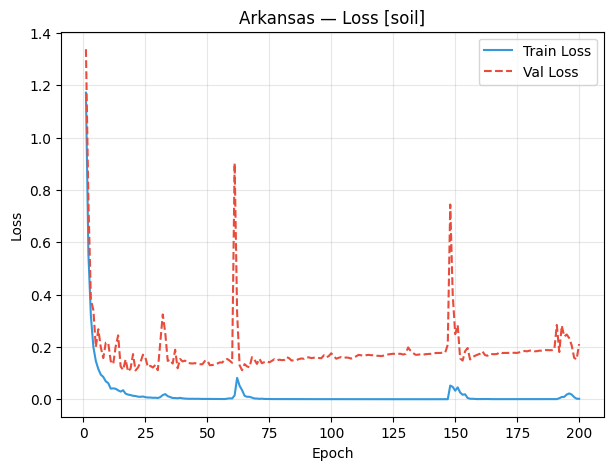
\includegraphics[width=\textwidth]{figures/arkansas_loss_soil.png}
    \caption{Arkansas — configuration \texttt{soil} (meilleure)}
    \label{fig:loss_ark_soil}
  \end{subfigure}
  \hfill
  \begin{subfigure}[b]{0.48\textwidth}
    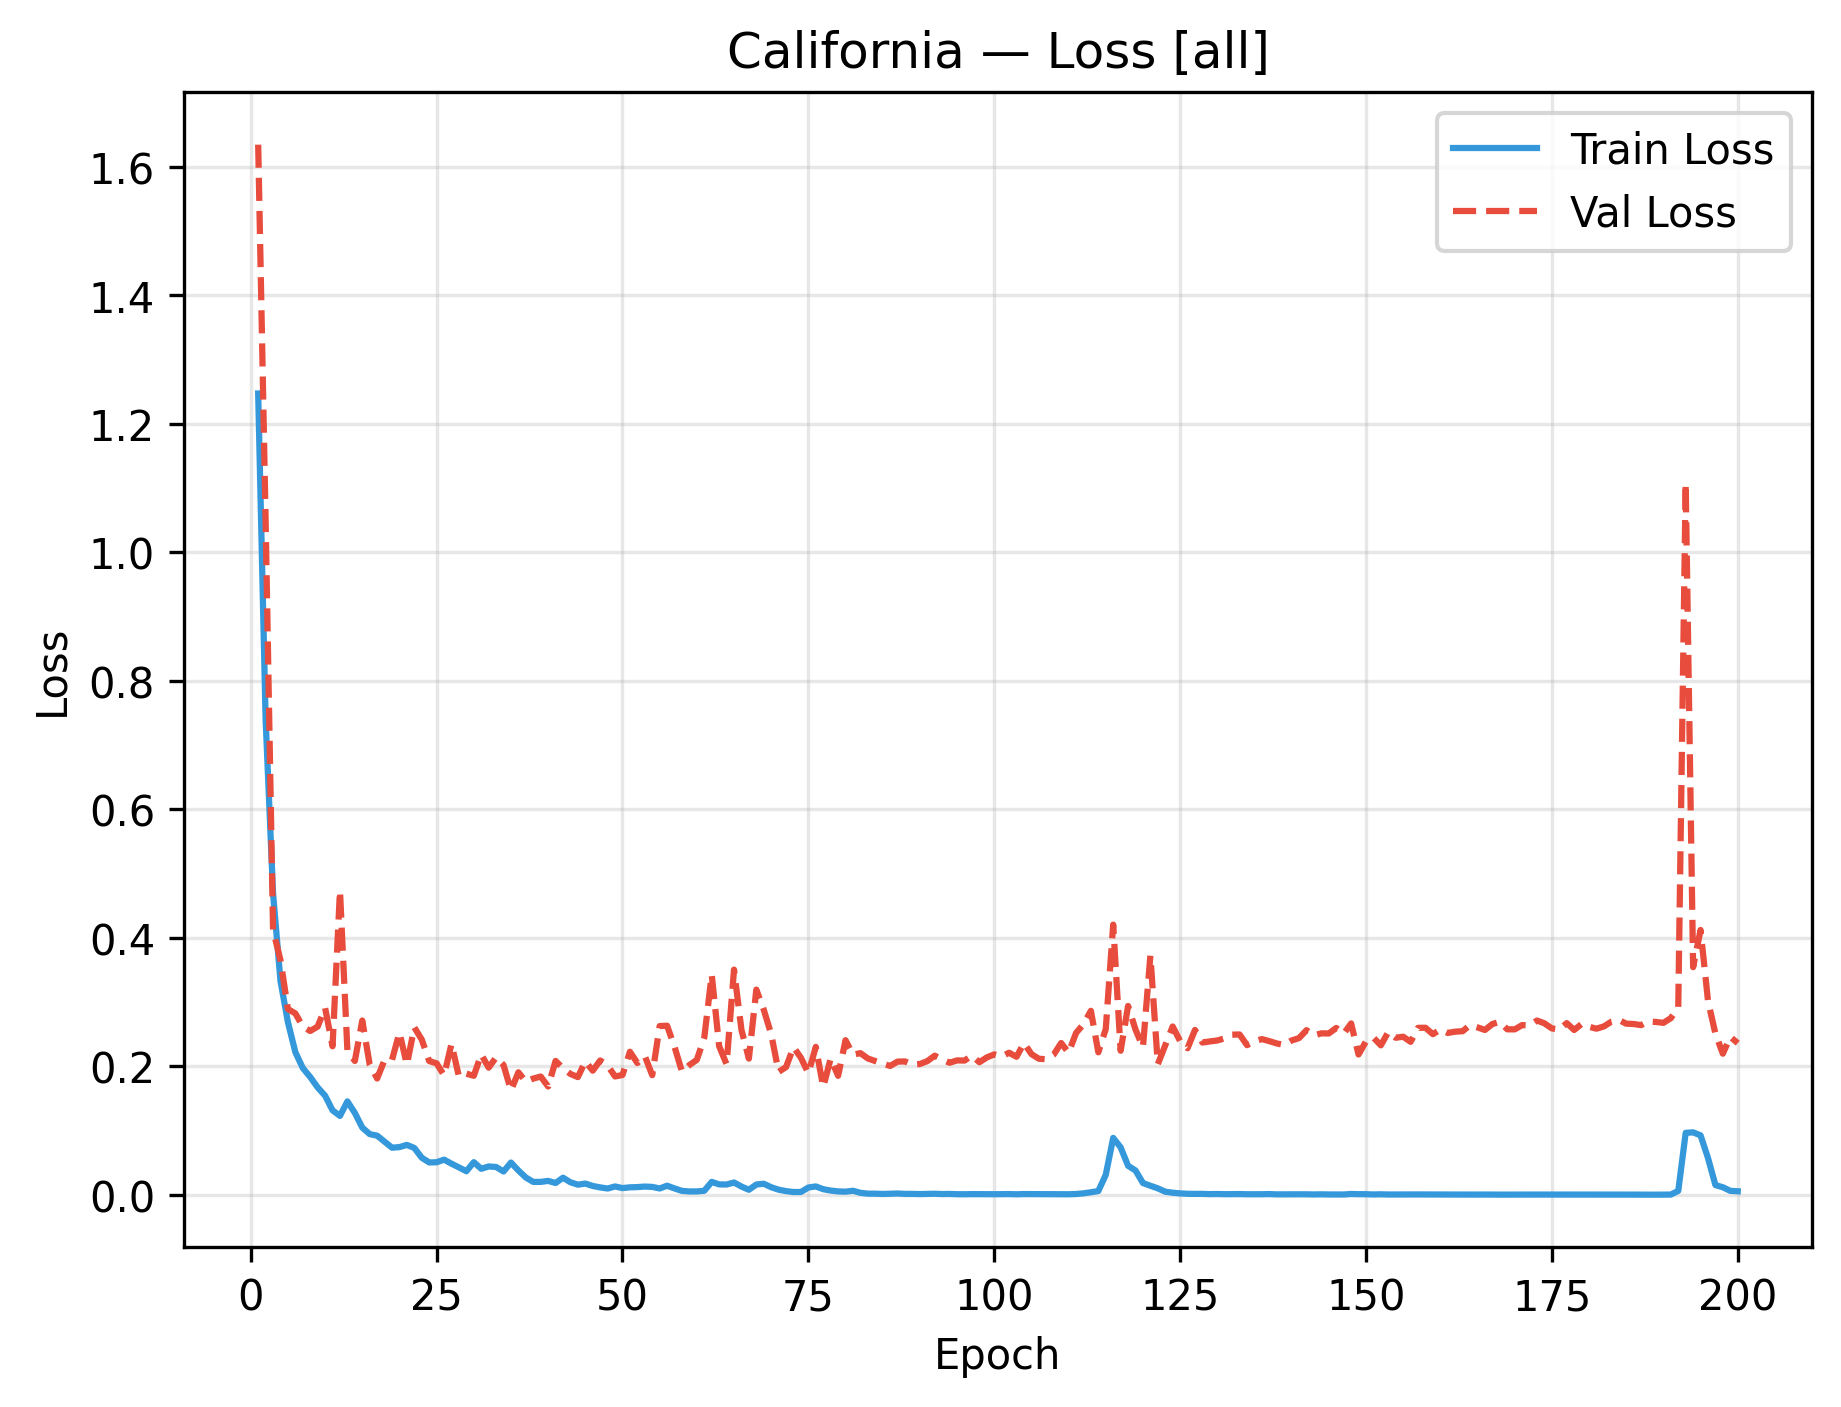
\includegraphics[width=\textwidth]{figures/California_all_loss.png}
    \caption{Californie — configuration \texttt{all} (meilleure)}
    \label{fig:loss_cal_all}
  \end{subfigure}
  \caption{Courbes d'apprentissage pour les meilleures configurations de covariables
  par région. La loss Arkansas descend régulièrement (faible surapprentissage) ;
  la loss Californie présente davantage d'oscillations, cohérent avec la plus grande
  complexité du jeu (6 classes, région géographiquement étendue).}
  \label{fig:loss_covars}
\end{figure}

\subsection{Matrices de confusion}

\begin{figure}[H]
  \centering
  \begin{subfigure}[b]{0.48\textwidth}
    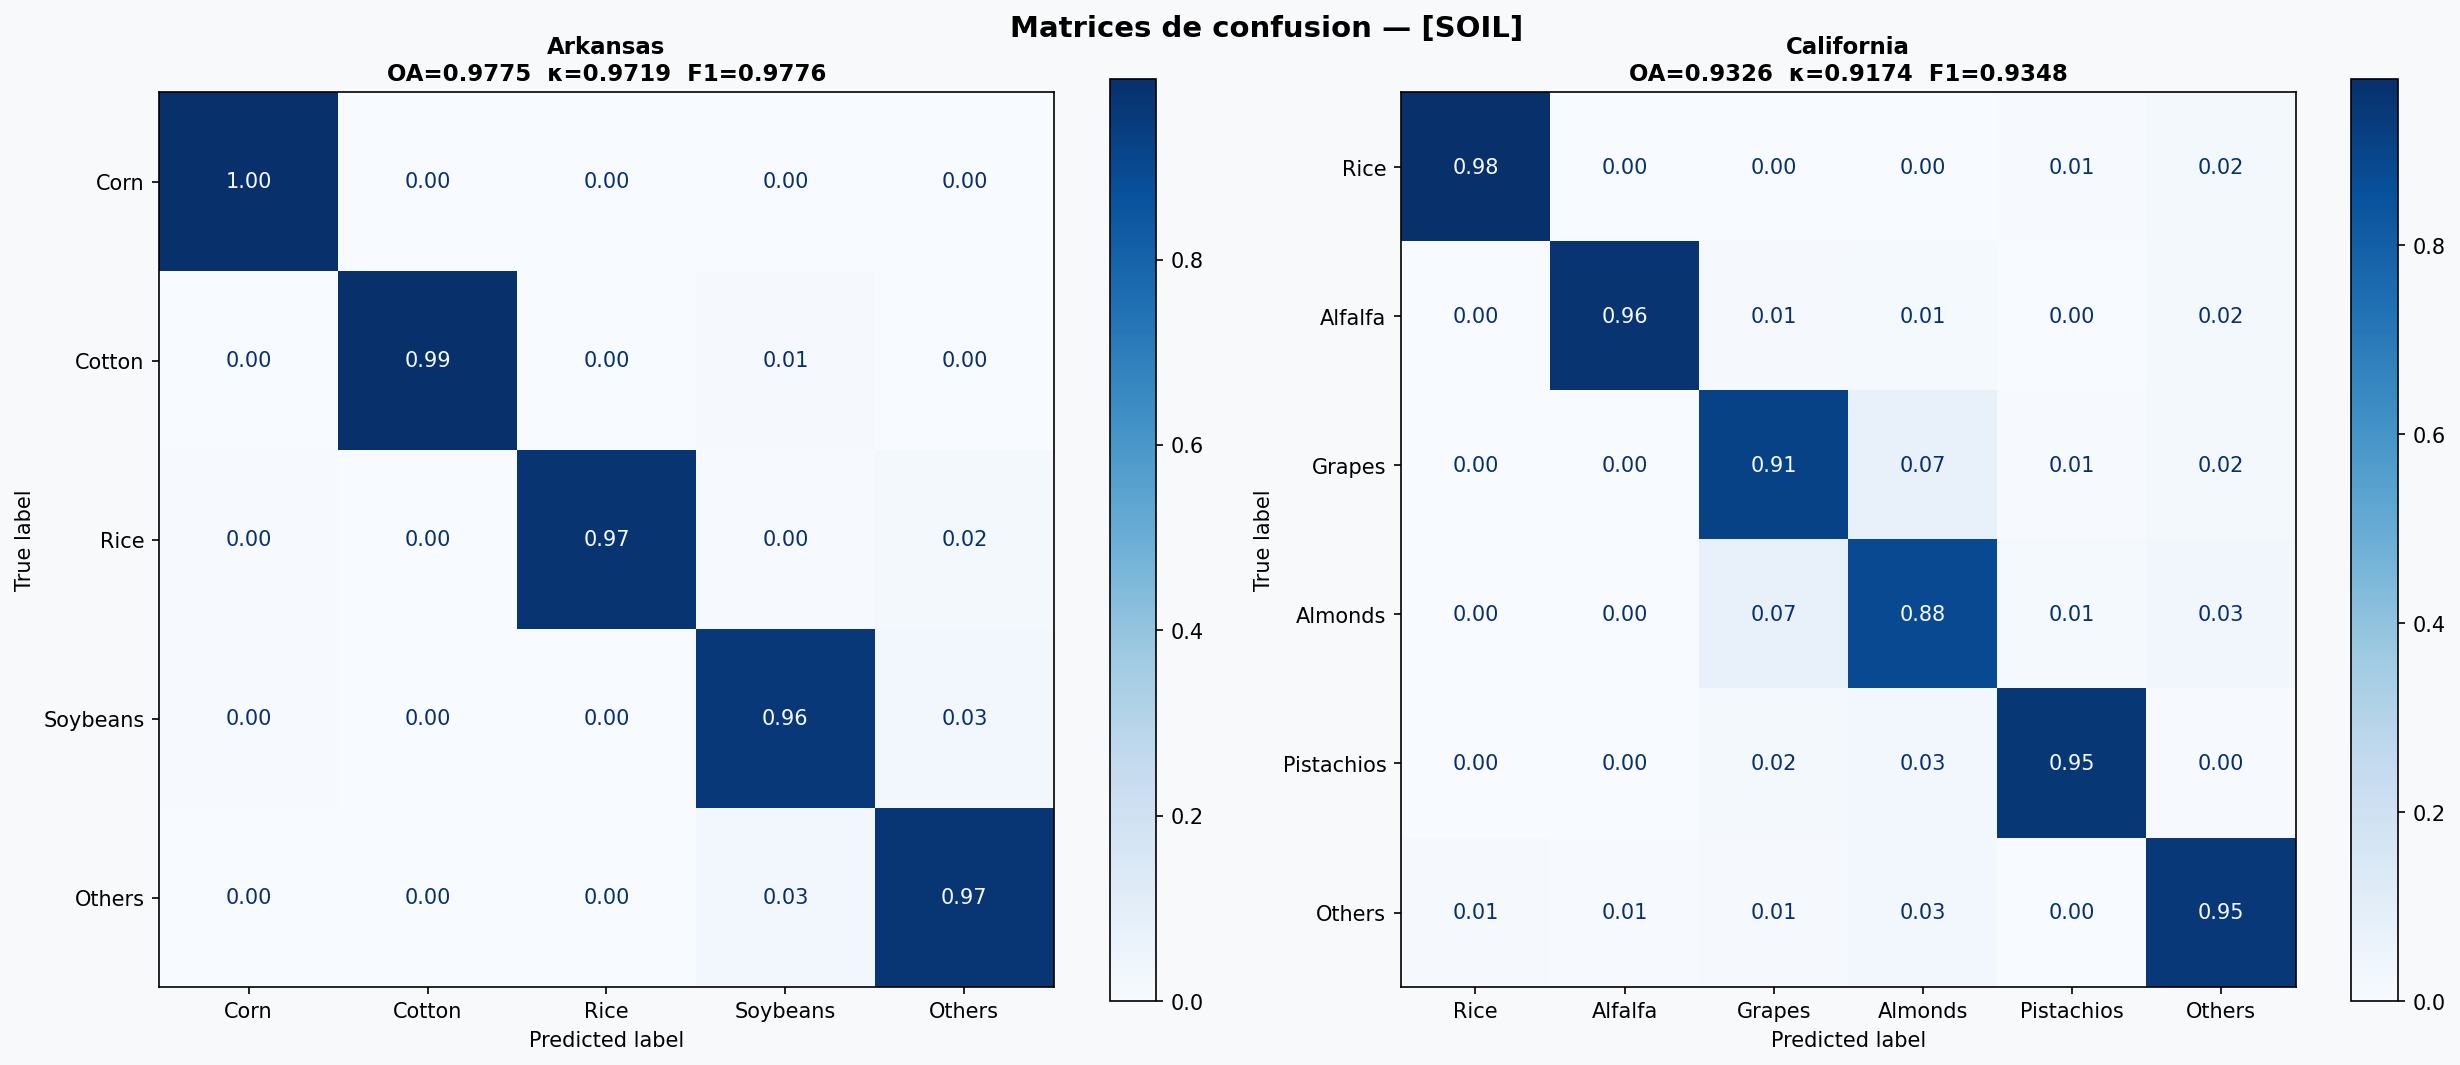
\includegraphics[width=\textwidth]{figures/confusion_comparison_soil.png}
    \caption{Arkansas — \texttt{soil} vs baseline}
    \label{fig:conf_ark_soil}
  \end{subfigure}
  \hfill
  \begin{subfigure}[b]{0.48\textwidth}
    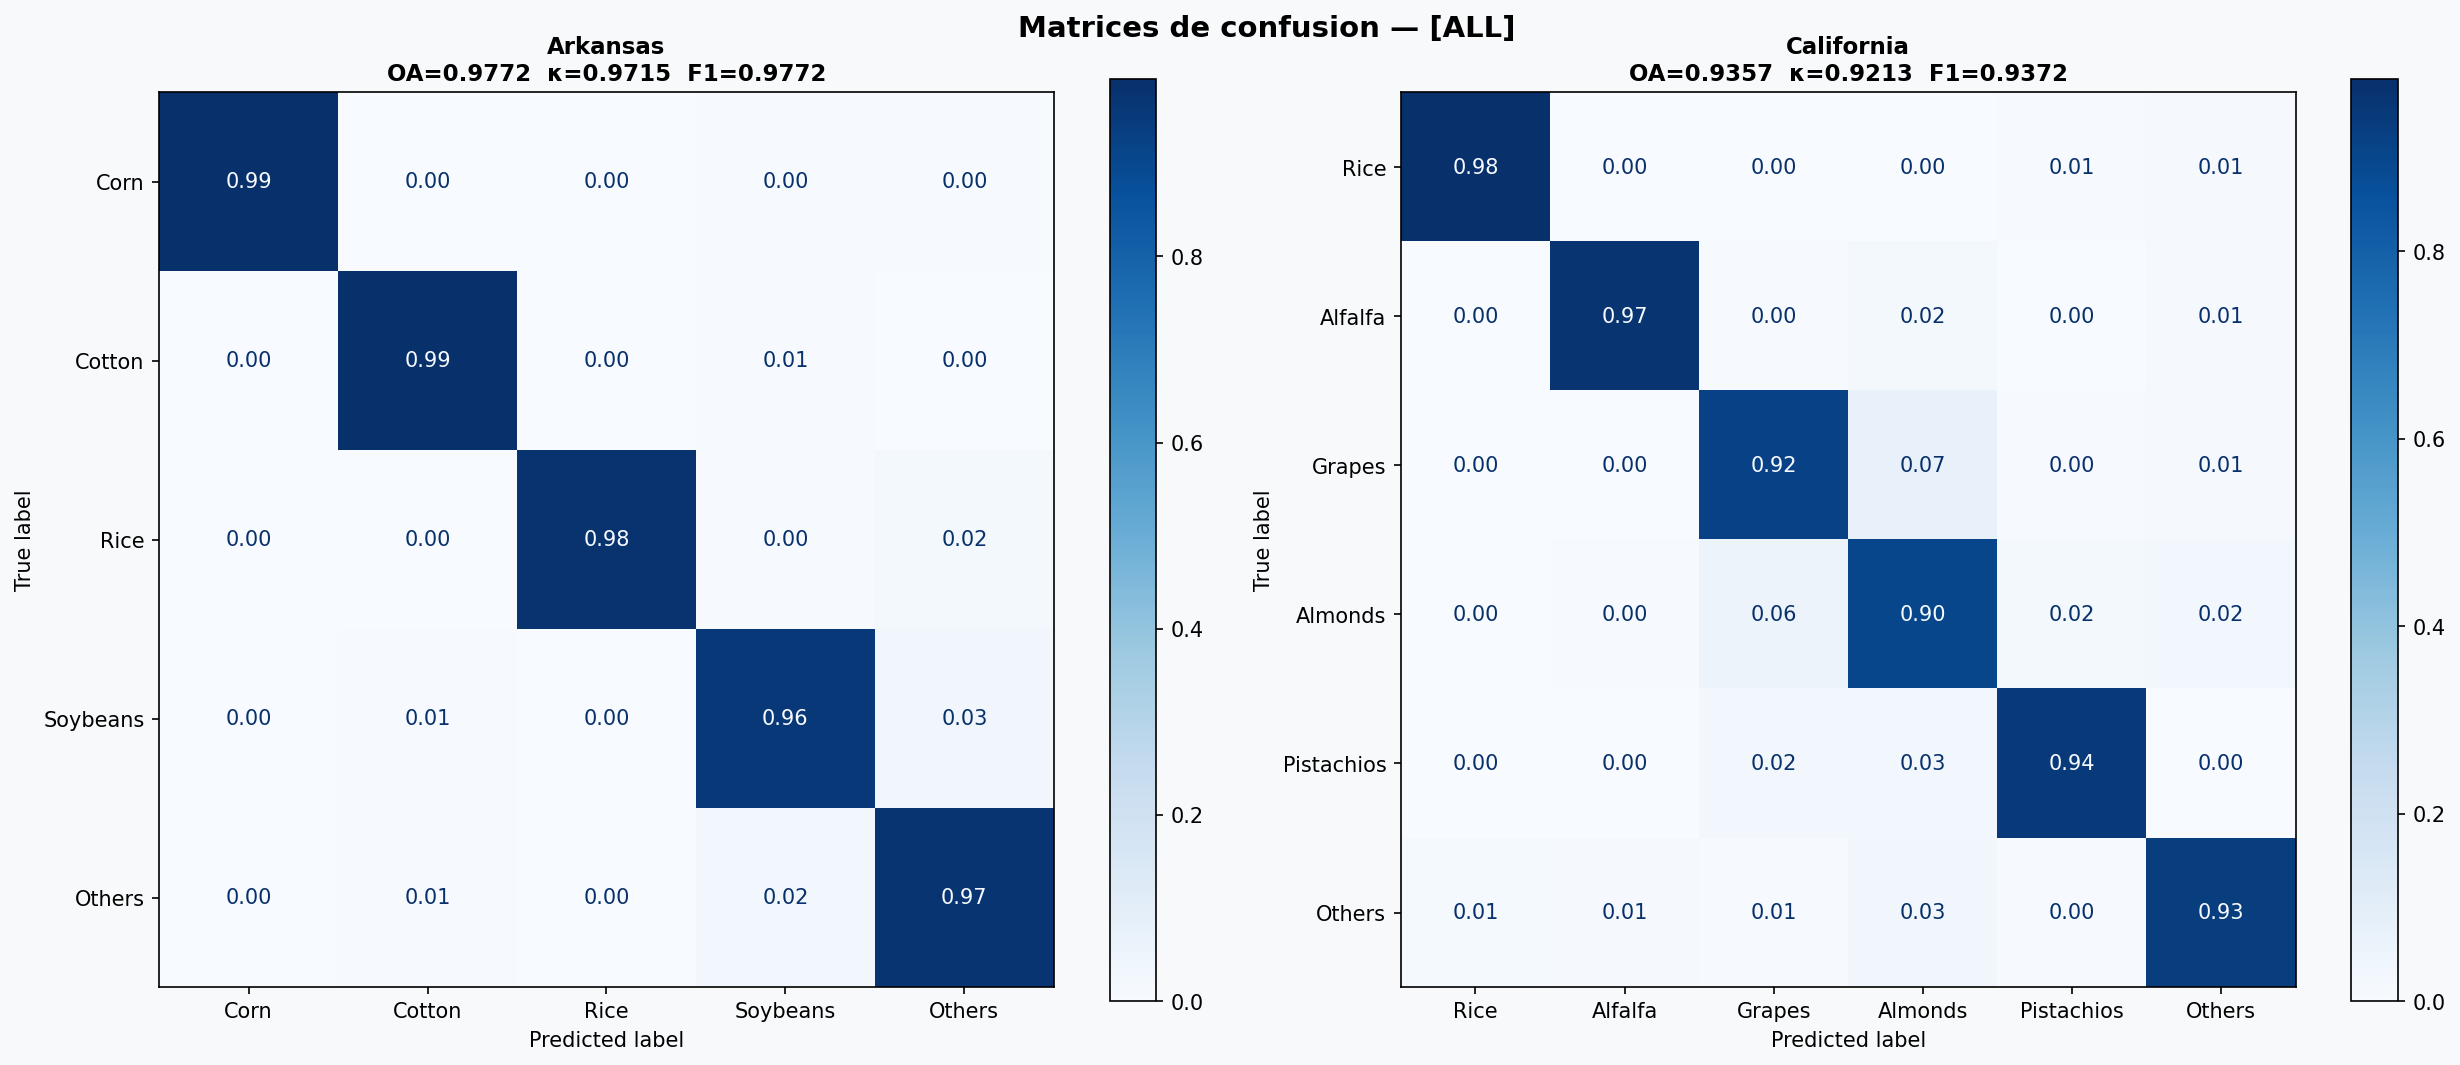
\includegraphics[width=\textwidth]{figures/confusion_comparison_all.png}
    \caption{Californie — \texttt{all} vs baseline}
    \label{fig:conf_cal_all}
  \end{subfigure}
  \caption{Matrices de confusion comparatives (MCTNet baseline vs meilleure configuration
  de covariables). En Arkansas, les covariables pédologiques réduisent principalement
  les confusions entre le riz et les autres céréales. En Californie, la combinaison
  complète améliore la discrimination des cultures pérennes (vigne, amandiers).}
  \label{fig:confusion_covars}
\end{figure}

\begin{figure}[H]
  \centering
  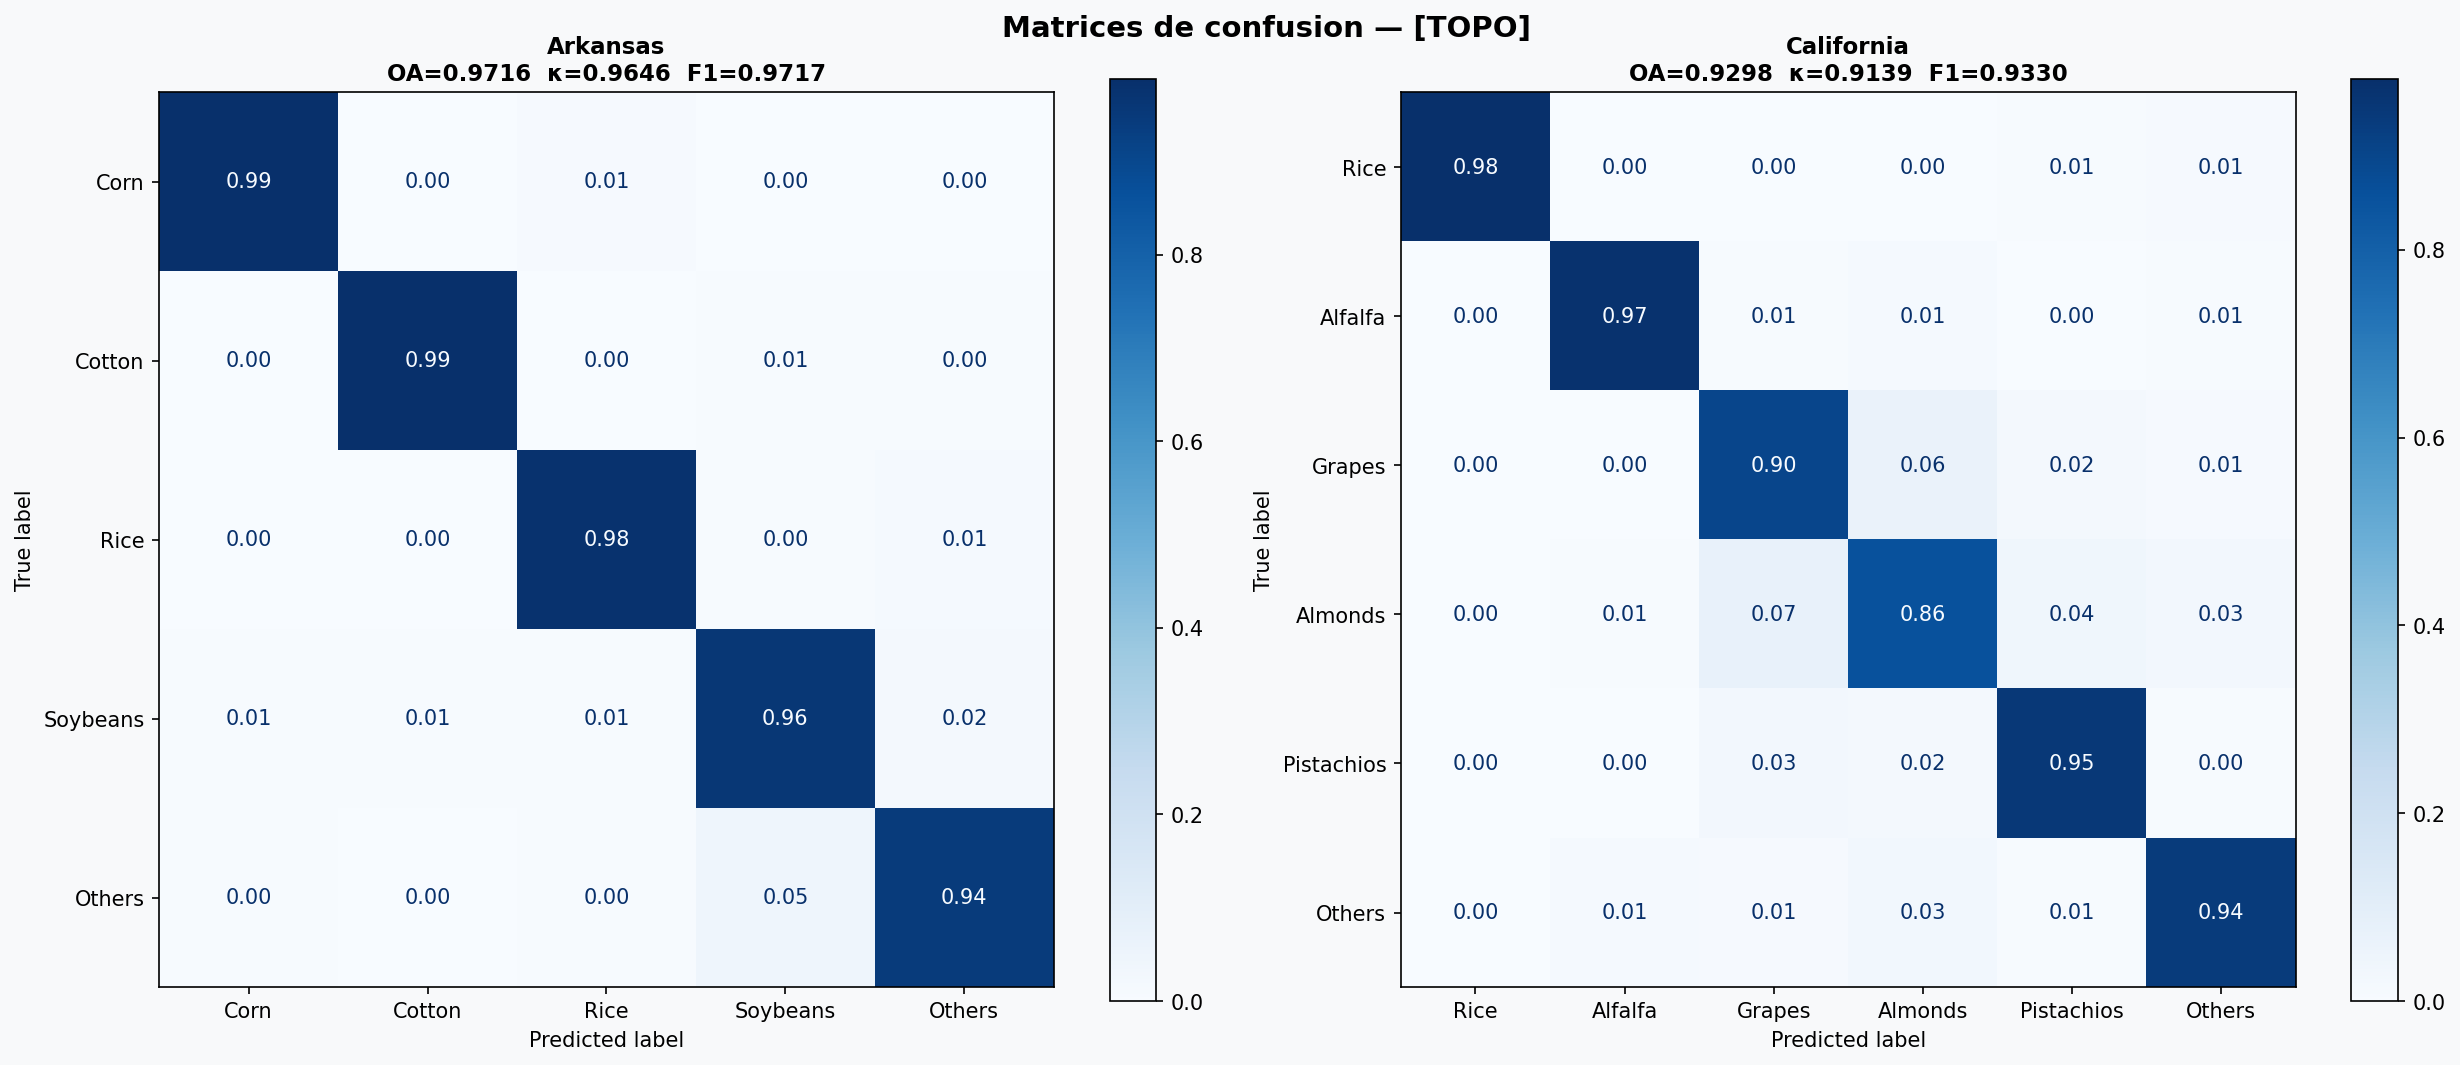
\includegraphics[width=0.6\textwidth]{figures/confusion_comparison_topo.png}
  \caption{Californie — configuration \texttt{topo} seul : la topographie introduit
  des confusions supplémentaires par rapport au baseline, confirmant son apport limité
  sans information climatique complémentaire.}
  \label{fig:conf_topo}
\end{figure}

\cleardoublepage
